\documentclass[tt3]{penoverslag}

%%% PACKAGES
\usepackage{lipsum}
\usepackage{gensymb}
\usepackage [dutch] {babel}
\usepackage{graphicx}
\usepackage{amsmath}
\usepackage{listings}
\usepackage{subcaption}
\usepackage[absolute]{textpos}
  \setlength{\TPHorizModule}{1cm}
  \setlength{\TPVertModule}{1cm}


\begin{document}

\team{Zilver} % teamkleur
\members{Sam Gielis\\
         Sophie Marien\\
         Toon Nolten\\
         Nele Rober\\
         Gerlinde Van Roey\\
         Maxim Van Mechelen} % teamleden

\maketitlepage

\newpage
%TODO De Doolhof en Het Doolhof nakijken voor consequente schrijfwijze. Gekalibreerd en gecalibreerd

\begin{abstract}
\label{ssec:Abstract}
Het P\&O-project heeft als doel vier autonome robots \textit{Team Treasure Trek} te laten spelen. Dit verslag beschrijft de invulling die team Zilver aan het project gaf.\\

De robot is voorzien van een lichtsensor, een infraroodsensor en een ultrasone sensor. Verder heeft de robot van een strip klittenband vooraan waarmee hij het voorwerp kan oprapen.
De robot kan een doolhof verkennen en hiervan een map bijhouden. Via RabbitMQ kunnen de robots en simulatoren met elkaar communiceren. Zo kunnen ze een map naar elkaar doorsturen om naar elkaar toe te rijden.\\

Een computerprogramma simuleert de werking van robots. Deze simulator kan vier robots tegelijk simuleren of kan in hybride vorm gebruikt worden (waarbij bijvoorbeeld \'e\'en fysieke en drie virtuele robots gebruikt worden). De gesimuleerde robots gedragen zich volledig analoog aan de fysieke robot.
\end{abstract}



%figuur robot
\begin{figure}[!hb]
\begin{textblock}{38}(5.4,16)
    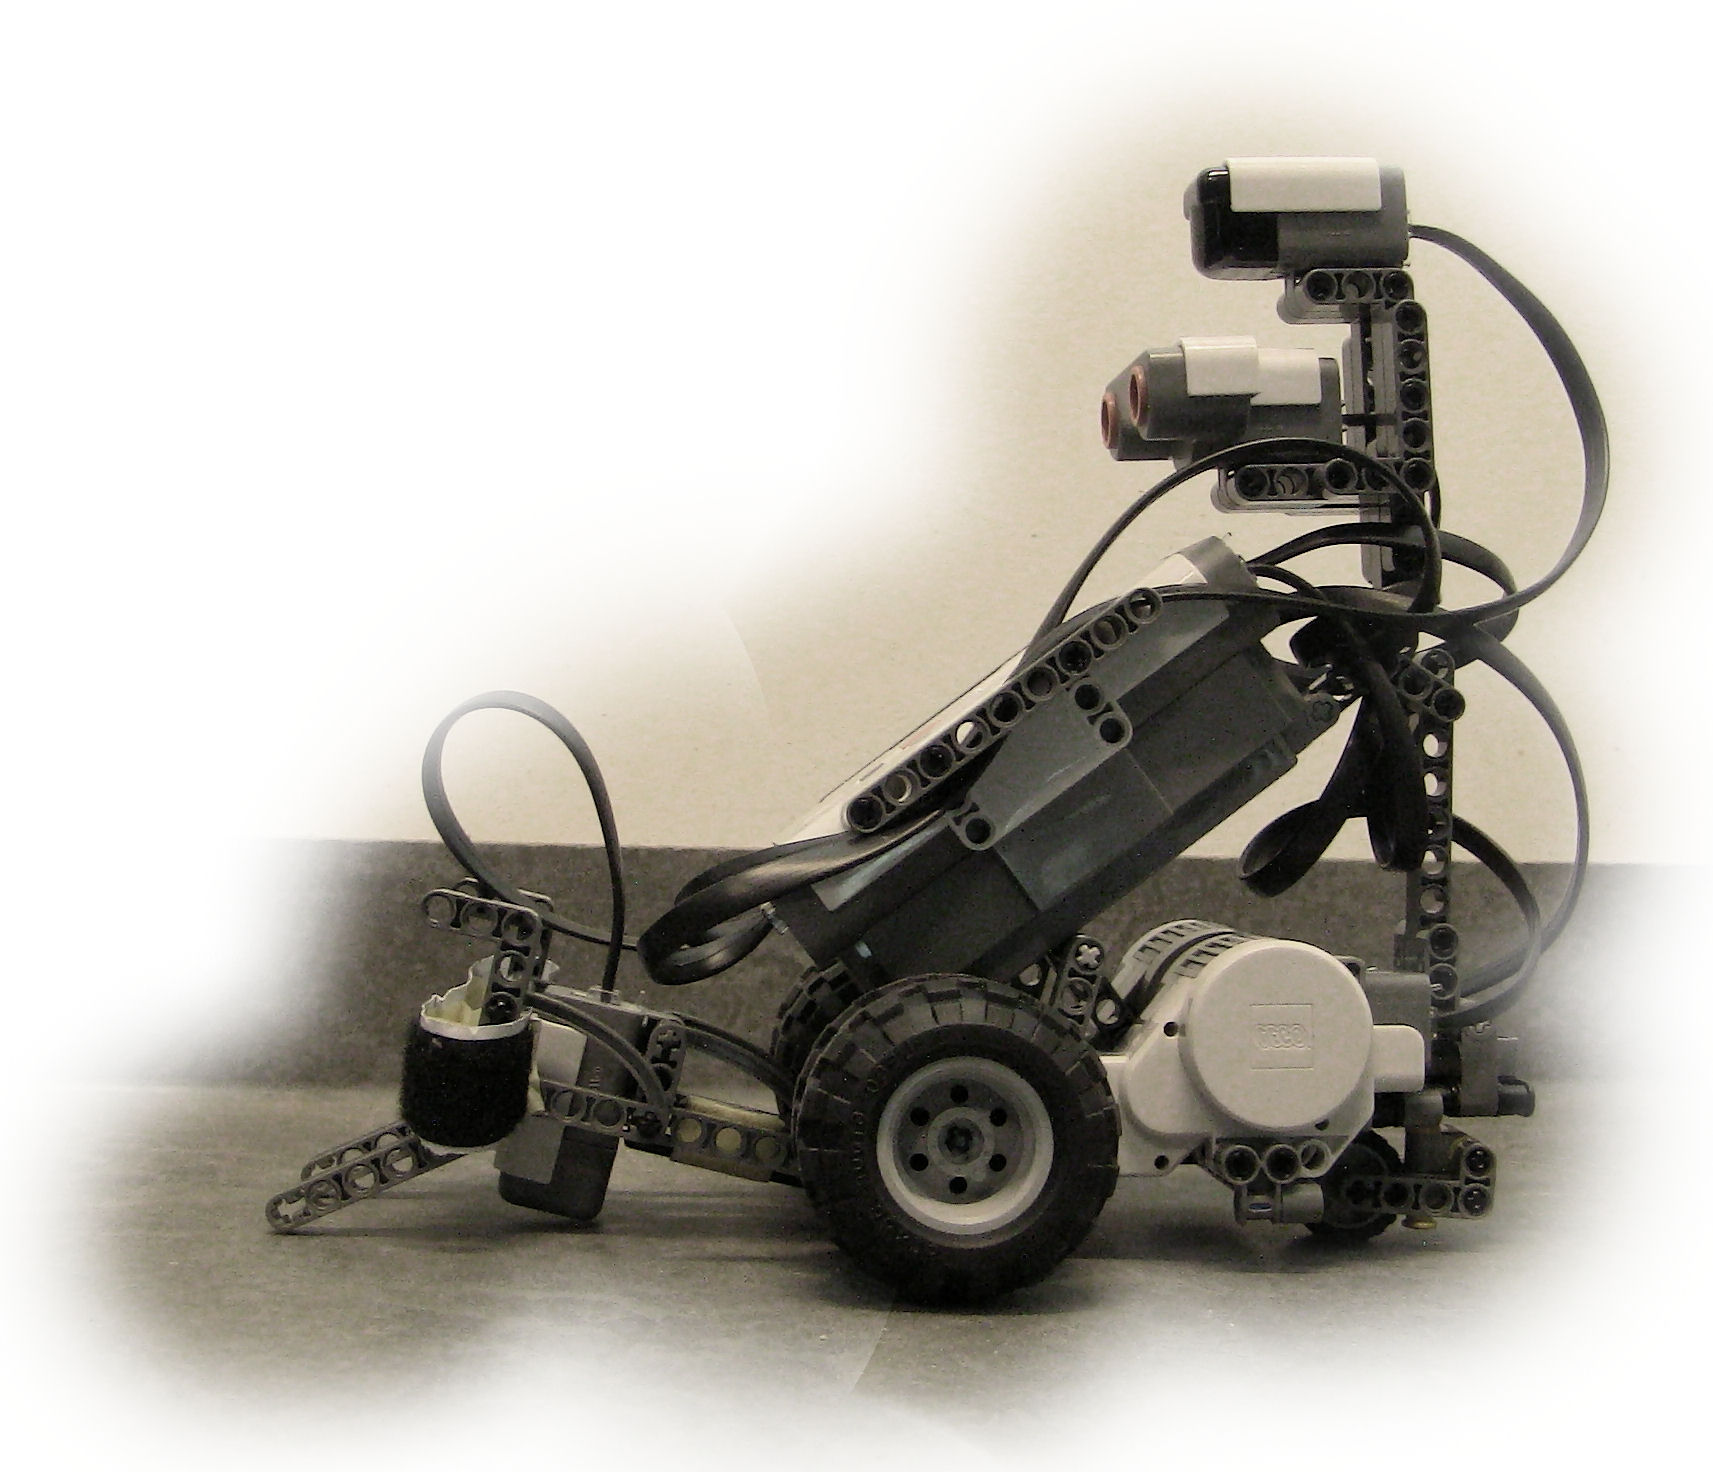
\includegraphics[width=0.38\textwidth]{robotFP}
    \label{fig:robotFP}
\end{textblock}
\end{figure}

\newpage
\setcounter{tocdepth}{3}
\tableofcontents
\newpage

% == INLEIDING == %
\section{Inleiding} % 4 ok
\label{ssec:Inl}
In het kader van het vak `Probleemoplossen en Ontwerpen: computerwetenschappen' wordt gewerkt rond autonome intelligente robots. Verschillende teams bouwen en programmeren een robot met behulp van LEGO Mindstorms. Deze robot moet uiteindelijk samen met drie andere robots volledig autonoom \textit{Team Treasure Trek} kunnen spelen.
De robots moeten hierbij in een onbekend doolhof op zoek naar een bepaald voorwerp (een wc-rol). Elke robot krijgt een eigen voorwerp toegewezen. Wanneer een robot zijn voorwerp gevonden heeft, komt hij te weten met welke robot hij moet samenwerken. Elk duo moet beide voorwerpen bij elkaar brengen. Het duo dat hier eerst in slaagt, wint.\\

Bij de derde demonstratie moet het volledige spel gespeeld kunnen worden. Dit kan met vier fysieke robots, met een combinatie van fysieke en virtuele robots of enkel met virtuele robots.

\section{Robot}
\label{ssec:Robot}

\subsection{Bouw Robot}
\label{ssec:Bouw}
LEGO Mindstorms biedt een bouwpakket voor een robot aan. Een NXT-microcomputer laat toe de robot te programmeren. Met behulp van leJOS kan dit in Java.

\subsubsection{Ontwerp}
\label{ssec:FysB}
Een infraroodsensor werd gemonteerd bovenop de robot. Doordat er een infraroodbal onder een wip ligt, kan de robot bepalen of de wip naar beneden staat. In dat geval wordt het infrarood licht immers geblokkeerd. De scheidsrechtercommissie speelde met het idee deze infraroodsensor ook te gebruiken voor robotdetectie, maar dit is er uiteindelijk niet doorgekomen.\\

Het voorwerp kan op verschillende manieren worden opgeraapt. Volgende opstellingen werden gebouwd en getest:

\begin{enumerate}
\item \textbf{Figuur~\ref{fig:robotOud1}}. De robot heft het voorwerp expliciet op met behulp van een extra motor. Deze opstelling maakt de robot te lang waardoor hij moeilijk kon draaien zonder tegen een muur te botsen. Er werd besloten de schep vooraan te plaatsen.
\item \textbf{Figuur~\ref{fig:robotOud2}}. Vooraan is niet genoeg plaats voor een extra motor, deze kon dus niet meer gebruikt worden. Een halve wc-rol leek een ideale vorm voor de schep. Na het voorwerp een aantal keer op te rapen, bleek dit echter niet altijd te werken.
\item \textbf{Figuur~\ref{fig:robotOud3}}. De robot neemt het voorwerp op met behulp van klittenband. De schep van lego zorgt ervoor dat het voorwerp niet over de grond sleept. Deze opstelling maakt de robot echter nog steeds te lang.
\item \textbf{Figuur~\ref{fig:robotBouw}}. %TODO huidige opbouw
\end{enumerate}


Het vorig ontwerp van de robot is aangepast. Uit de vorige demo bleek dat de robot bij het oprijden en afrijden van de wip heel schokkerig beweeg, ook wanneer de robot draaide of sneller wou rijden. Voor deze demo hebben we de robot helemaal terug opnieuw in elkaar gestoken. De wielen zijn verder uit elkaar gezet zodat de robot breeder wordt. De NXT is schuin erop gezet omdat het zo goed uit kwam om te monteren. Het bijkomend voordeel dat we hierbij hadden, was dat er dan aan de achterkant genoeg plaats was om een schep voor het voorwerp te monteren. De schep heeft ook een motor gekregen. Initieel staat de schep naar boven en deze wordt naar beneden gedaan wanneer de robot het voorwerp moet oprapen.  Dit nieuwe ontwerp betekende wel dat er opnieuw getest moest worden en dat de sensoren terug opnieuw gekalibreerd moesten worden.

De infrarood- en ultrasone sensor staan vast gemonteerd op de robot. De lichtsensor werd scharnierend gemonteerd. Wanneer het hefboomsysteem de wip raakt, kantelt het omhoog. Zo kan de robot vlot de wip op.

%Figuur~\ref{fig:robotDetail} geeft details van de schep, de wielen en de sensoren.

% bouw robot: oude ontwerpen
\begin{figure}
\centering
	\begin{subfigure}[h]{0.325\textwidth}
	\centering
		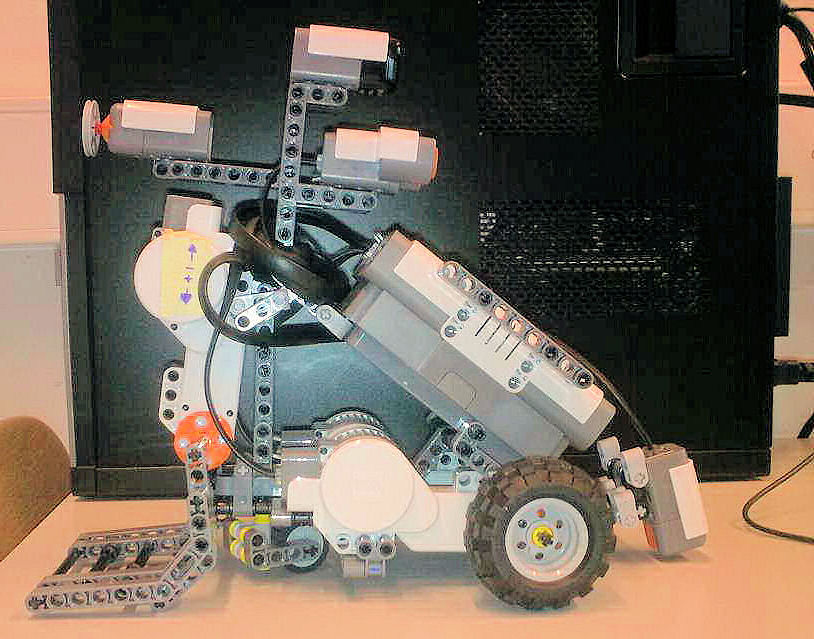
\includegraphics[width=\textwidth]{robotOud1}
		\caption{opstelling 1}
		\label{fig:robotOud1}
	\end{subfigure}
	\begin{subfigure}[h]{0.325\textwidth}
		\centering
		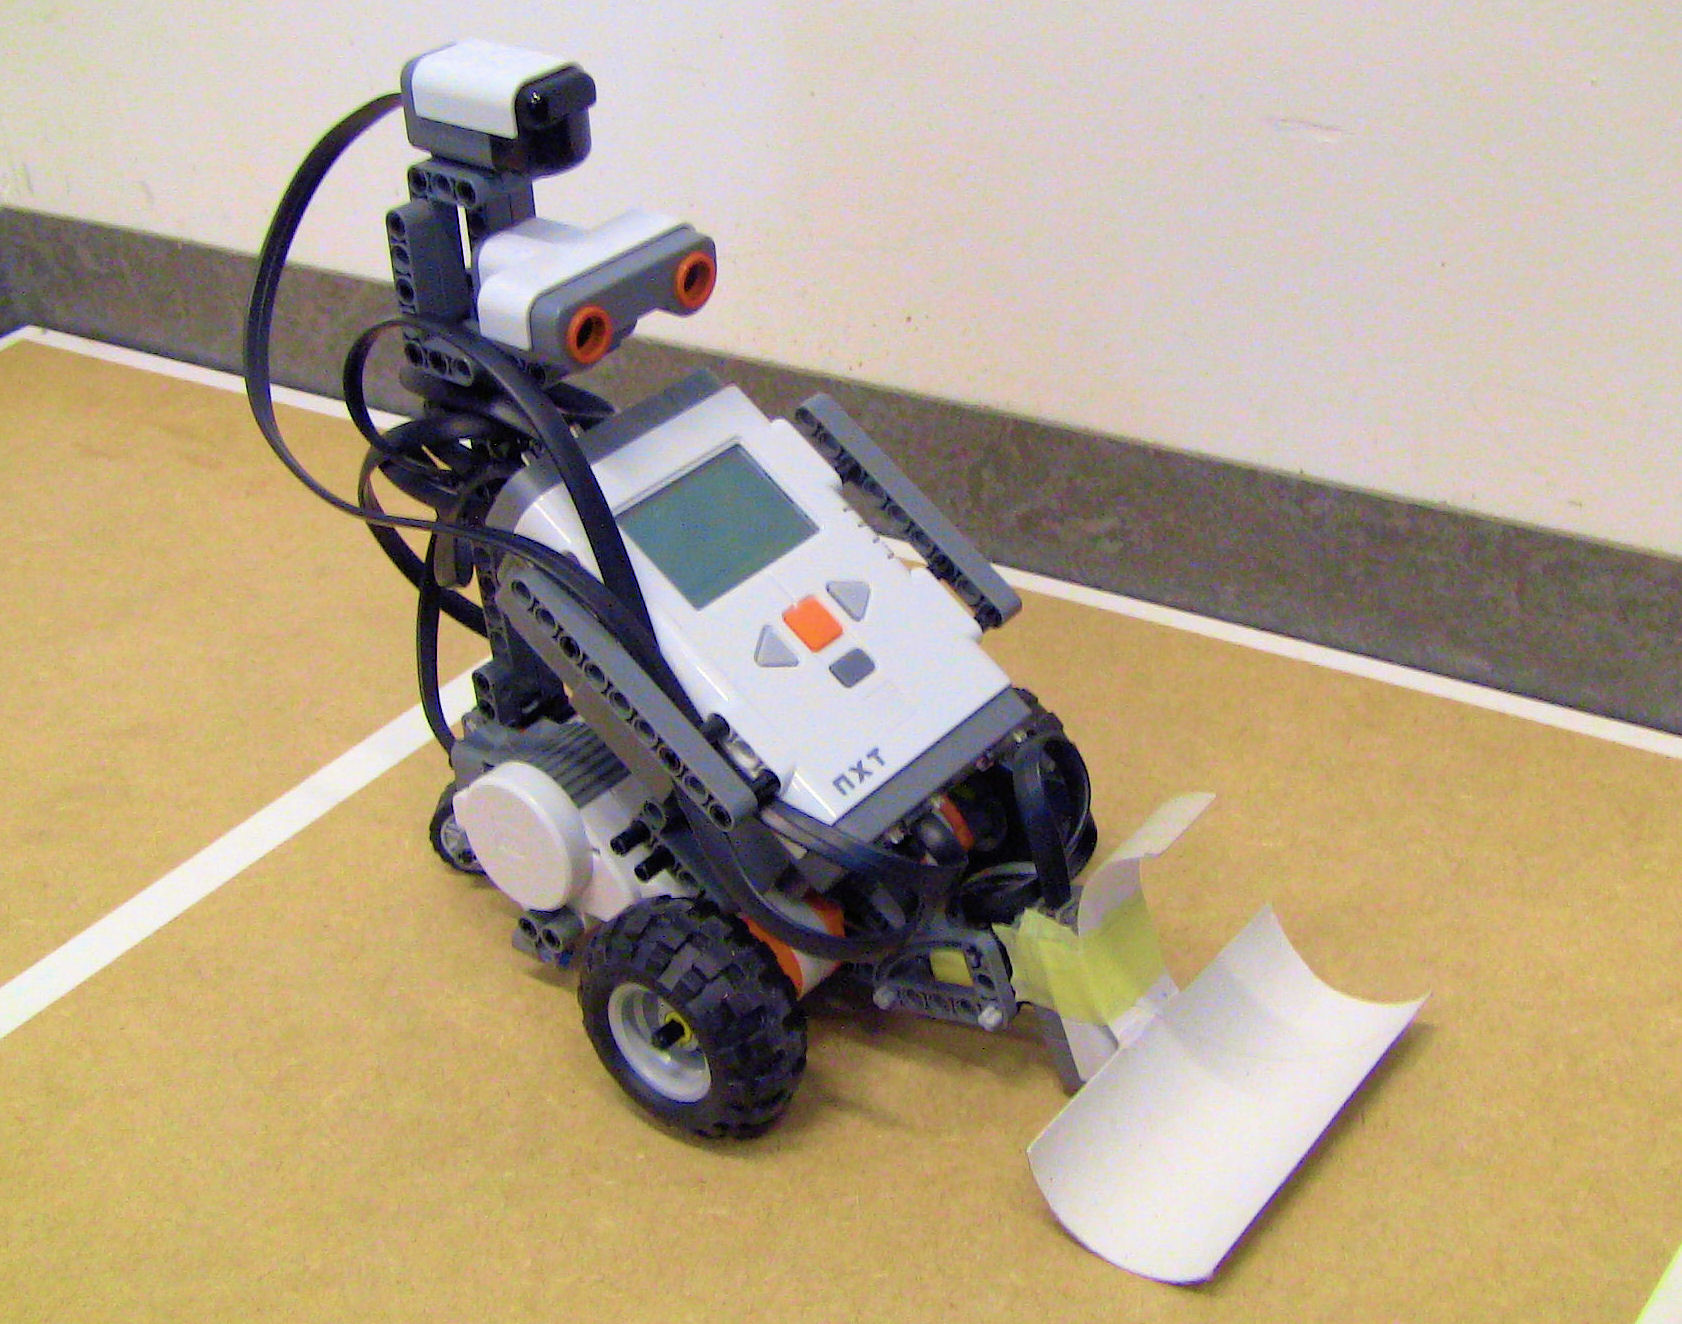
\includegraphics[width=\textwidth]{robotOud2}
		\caption{opstelling 2}
		\label{fig:robotOud2}
	\end{subfigure}
	\begin{subfigure}[h]{0.325\textwidth}
		\centering
		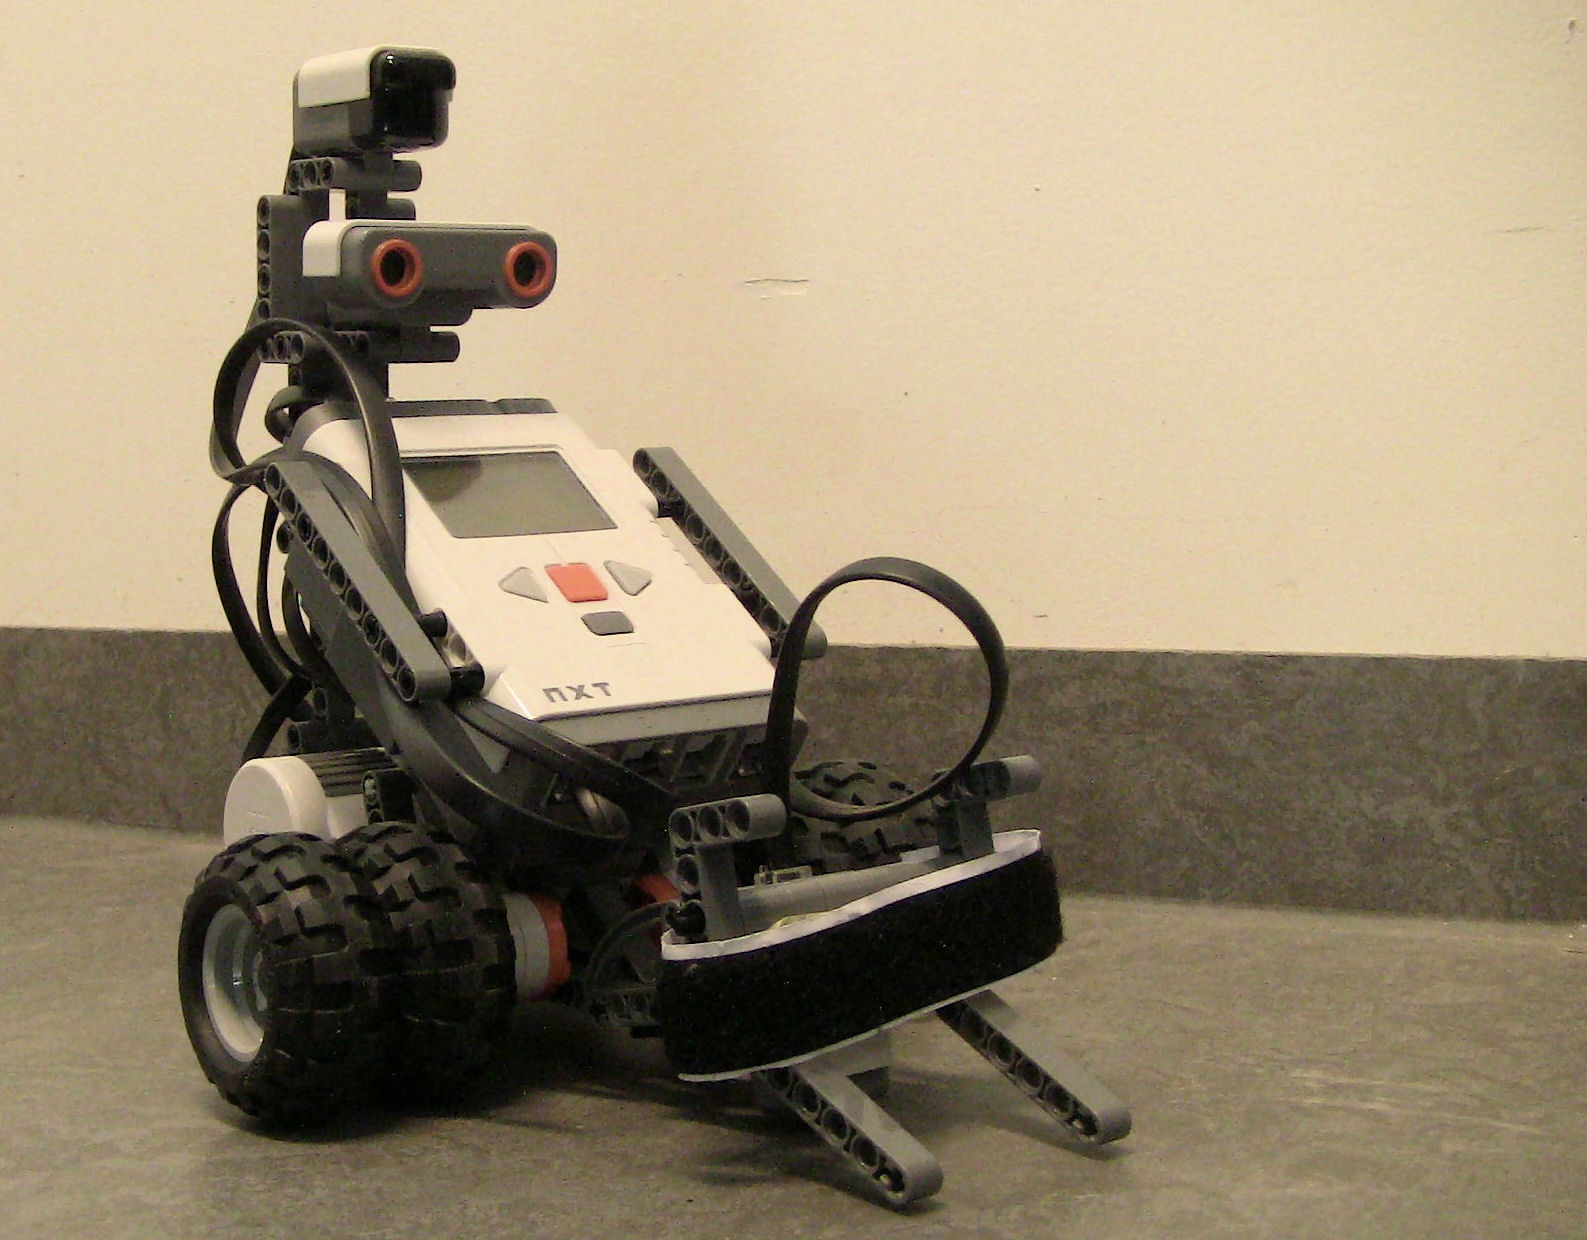
\includegraphics[width=\textwidth]{robotOud3}
		\caption{opstelling 3}
		\label{fig:robotOud3}
	\end{subfigure}
\caption{Alternatieve ontwerpen.}
\label{fig:robotOud}
\end{figure}

% bouw robot
\begin{figure}
\centering
	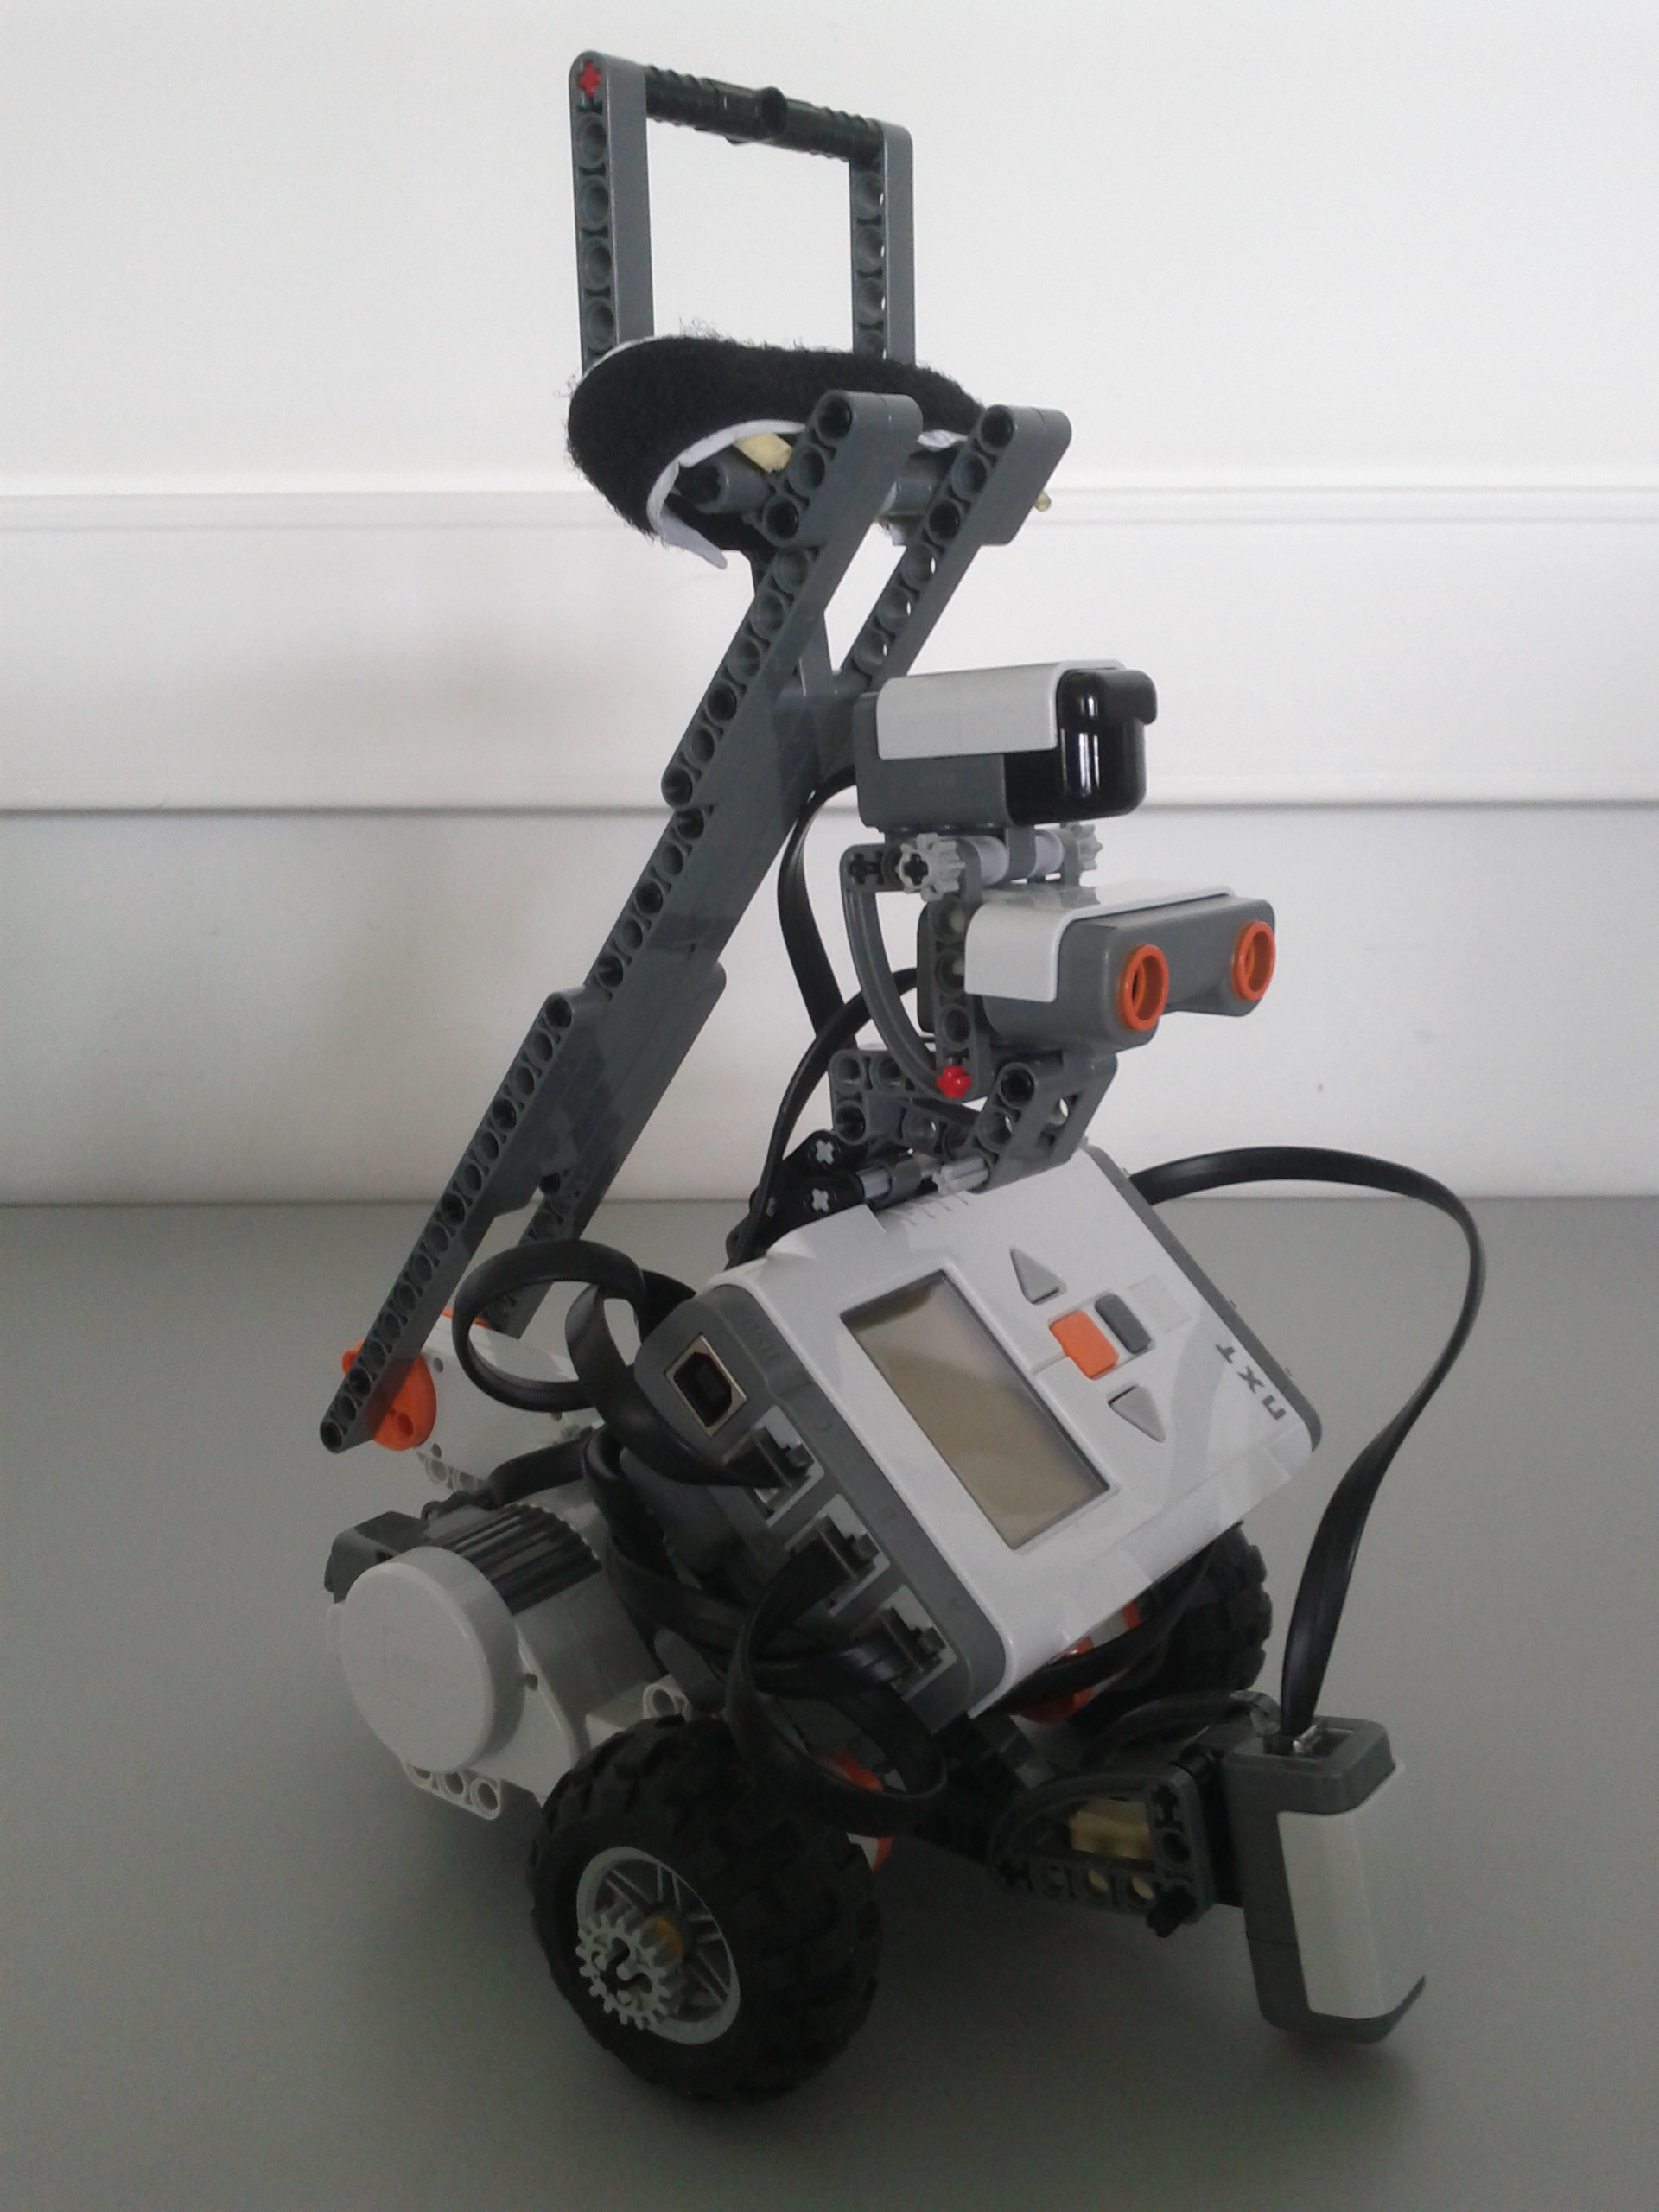
\includegraphics[width=0.5\textwidth]{robotNieuw}
\caption{Het huidige ontwerp.}
\label{fig:robotBouw}
\end{figure}

% details robot
\begin{figure}
\centering
	\begin{subfigure}[h]{0.325\textwidth}
	\centering
		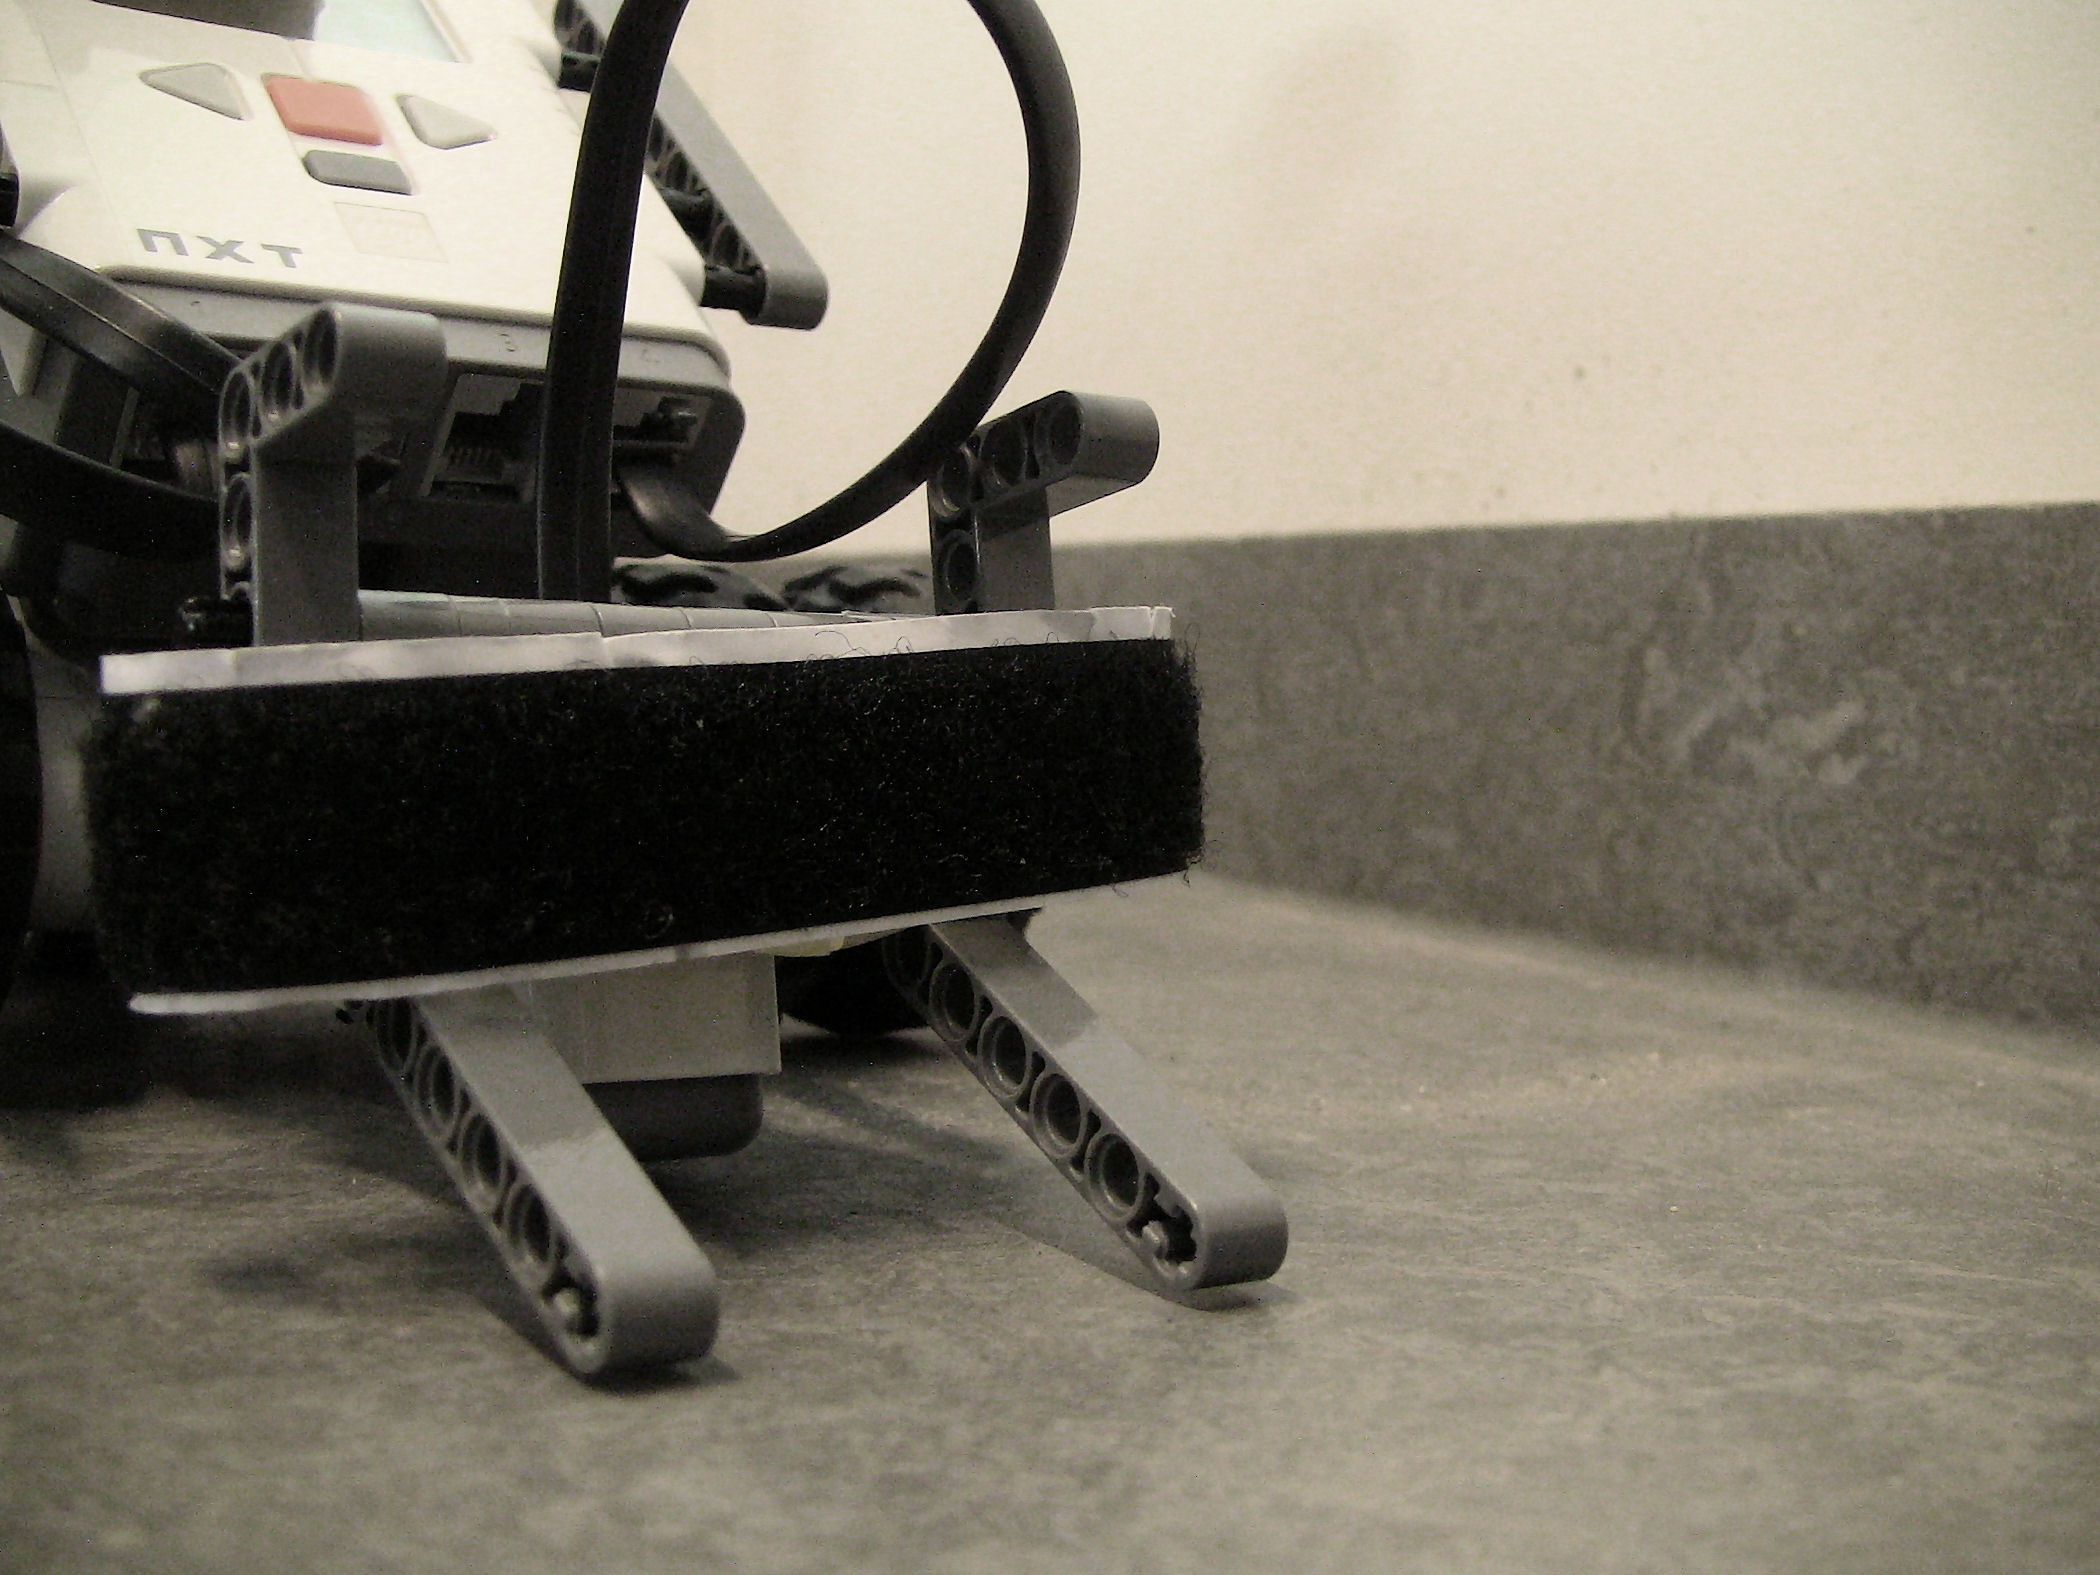
\includegraphics[width=\textwidth]{robotSchep}
		\caption{schep}
	\end{subfigure}
	\begin{subfigure}[h]{0.325\textwidth}
		\centering
		\includegraphics[width=\textwidth]{robotWielen}
		\caption{wielen}
	\end{subfigure}
	\begin{subfigure}[h]{0.325\textwidth}
		\centering
		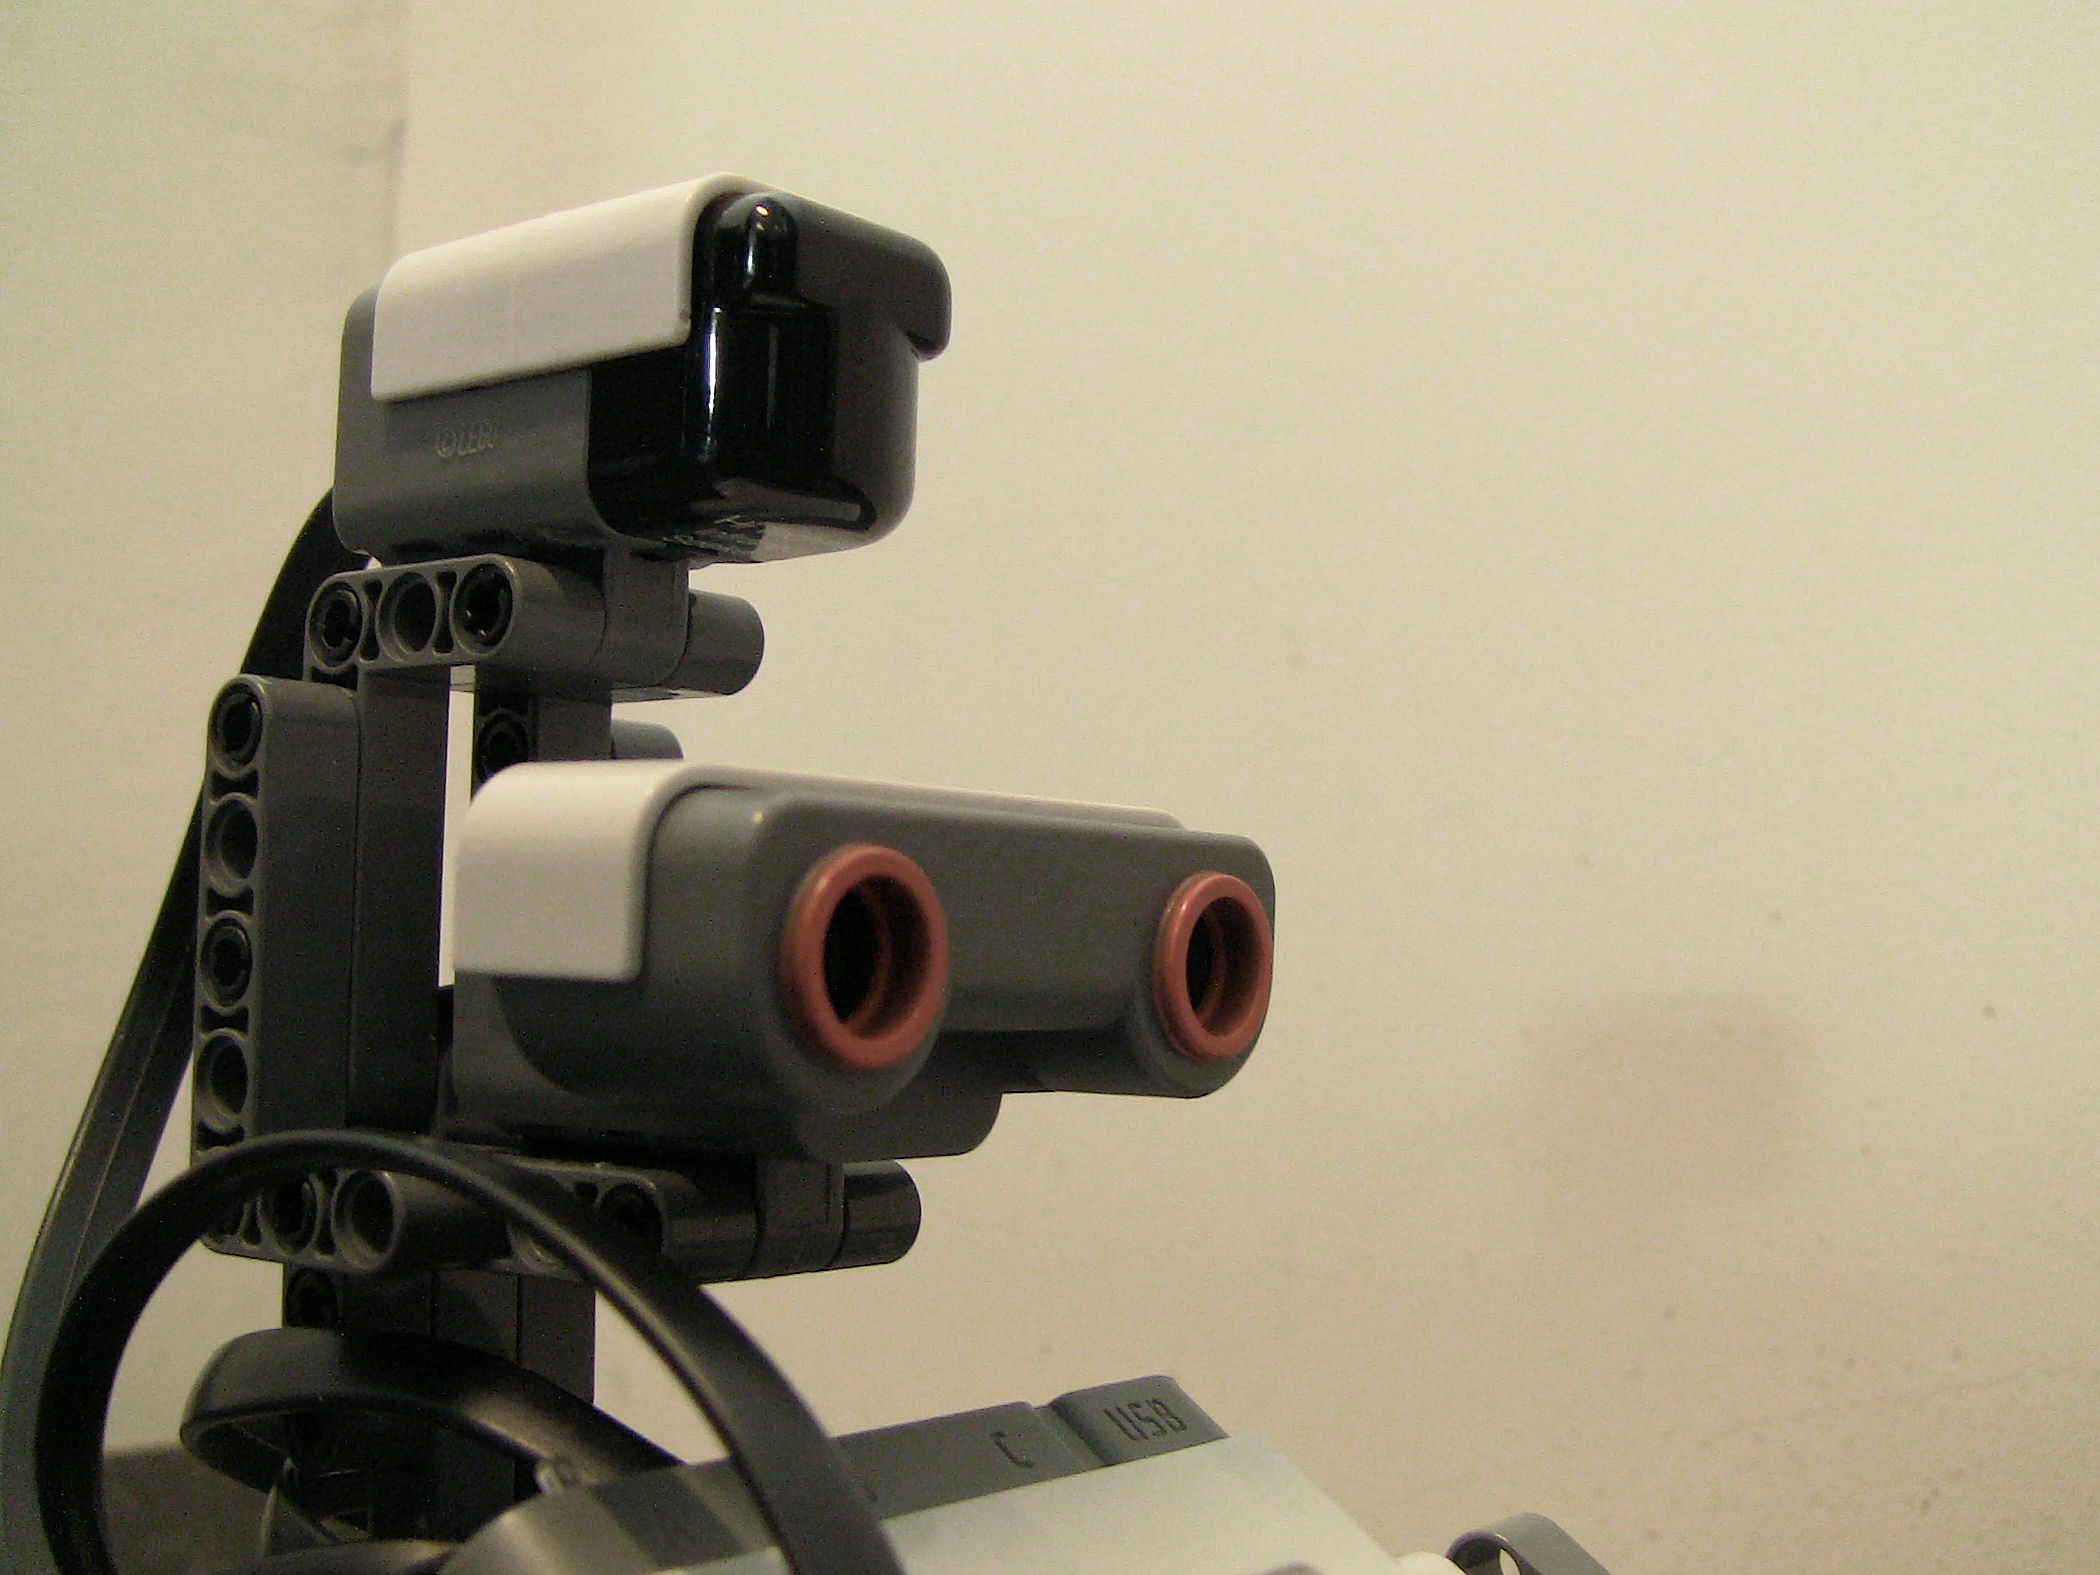
\includegraphics[width=\textwidth]{robotSensoren}
		\caption{infrarood- en ultrasone sensor}
	\end{subfigure}
\caption{Details van de robot.}
\label{fig:robotDetail}
\end{figure}

\subsection{Kalibratie}
\label{ssec:Kalib}
%TODO testresultaten
\subsubsection{Infraroodsensor}
\subsubsection{Ultrasone sensor}
\subsubsection{Lichtsensor}
\subsubsection{Druksensor}

% == ALGORITMES == %
\section{Algoritmes}
\label{sec:Algo}

\subsection{Verkennen doolhof}
\label{ssec: verkenDool}
% == robot aligneren == %
\subsubsection{Positie en ori"entatie corrigeren}
\label{ssec:AlgoAllign}
Het is niet mogelijk de robot perfect 100\% nauwkeurig te doen rijden. De motoren kunnen immers maar tot een bepaalde nauwkeurigheid ingesteld worden. Om de besturing toch betrouwbaar te maken is het nodig de robot af en toe te aligneren. Dit gebeurt bij elke tegel. %TODO klopt dit????
De methode bestaat uit twee basisalgoritmes: op basis van de witte lijn (sectie~\ref{ssec:AlgoAllignWit}) en op basis van de muren (sectie~\ref{ssec:AlgoAllignMuur}).

\begin{description}


\item \textbf{Aligneren op basis van een witte lijn}\\
\label{ssec:AlgoAllignWit}
De robot rijdt vooruit tot de lichtsensor wit detecteert. Hij rijdt verder tot de sensor weer bruin detecteert. Na een tweede check van de sensor stop de robot. Hij staat dan net over de witte lijn. De robot rijdt nog x cm vooruit zodat de wielas net boven de witte lijn staat.
Vervolgens draait de robot om zijn as tot de lichtsensor weer wit detecteert.
%TODO x

\begin{enumerate}
	\item rij vooruit tot je een witte lijn tegenkomt
	\item rij traag vooruit tot je over de lijn bent
	\item kijk een tweede keer of de ondergrond wel echt wit is; stop indien dit het geval is
	\item rij vooruit tot de wielas perfect boven de witte lijn staat
	\item draai om de as naar rechts tot de lichtsensor wit meet
	\item je staat nu perfect volgens de witte lijn: aligneer op basis van muren
	\item draai 90° terug; je staat nu in het midden van de witte lijn, loodrecht erop
\end{enumerate}

\item \textbf{Aligneren op basis van muren}\\
\label{ssec:AlgoAllignMuur}
Dit algoritme wordt enkel uitgevoerd wanneer de robot volgens een witte lijn staat. Het algoritme werkt als volgt:

\begin{enumerate}
	\item wanneer de ultrasone sensor meer dan x bedraagt: er staat geen muur voor je %TODO x
	\item wanneer de ultrasone sensor minder dan x en meer dan y bedraagt: rij achteruit tot hij y bedraagt %TODO y
	\item wanneer de ultrasone sensor minder dan y bedraagt: rij vooruit tot hij y bedraagt
\end{enumerate}

\end{description}


% == barcoes lezen == %
\subsubsection{Barcodes lezen}
\label{ssec:AlgoBar}
%TODO het lees-algoritme

Wanneer de gevonden barcode een voorwerp aanduidt, weet de robot dat de volgende tegel een ´dead-end' is zonder deze te moeten bezoeken. Deze tegel wordt automatisch toegevoegd aan de map en ingesteld als `verkend'.
Analoog voor een barcode die een wip aanduidt: de volgende drie tegels, waarvan er twee een wip bevatten, worden automatisch toegevoegd aan de map.

% === WIP === %
\subsubsection{Wip}
\label{ssec:AlgoWip}
Wanneer de robot een wip tegenkomt, zal hij deze in eerste instantie niet nemen. De robot zal eerst alle tegels aan deze kant van de wip verkennen. De kans is immers vrij groot dat hij de andere kant van de wip tegenkomt zonder deze te moeten oversteken. Wanneer alle tegels in de queue verkend zijn, behalve diegene die bereikbaar zijn via een wip, zal de robot wel over de wip rijden. De robot rijdt dan naar die wip die het dichtst bij is \'en die toegang geeft tot onverkende tegels.


% == zoeken van het voorwerp == %
\subsection{Zoeken van het voorwerp} %
\label{ssec:AlgoZoek}
Om het voorwerp te vinden moet de robot aanvankelijk het doolhof verkennen. In de loop van het eerste semester werd hiervoor een algoritme ontwikkeld. Dit werd toen verder geoptimaliseerd in volgende stappen: 

\begin{enumerate}
\item basisalgoritme: draai bij elke tegel vier keer (eindig in startori\"entatie) en neem de laatste tegel in de queue als volgende tegel.
\item neem steeds de buur die met het minst aantal rotaties bereikt kan worden als volgende tegel.
\item draai bij elke tegel slechts drie keer (eindig niet meer in startori"entatie).
\item kijk muren die vanuit een naburige tegel reeds gedetecteerd werden  niet nog eens na.
\item tegels waarvan de vier zijden al gekend zijn en waaraan drie muren grenzen, worden niet meer bezocht (`dead-ends' kunnen onmogelijk barcodes bevatten, dus dit is geen probleem)
\end{enumerate}

Bij de start van het tweede semester werd besloten een extra optimalisatie (6) toe te voegen. Deze geeft prioriteit aan `dead-ends'. Een voorwerp kan zich immers enkel bevinden op een `dead-end', voorafgegaan door een `straight' met een barcode. Onderstaande testen (sectie~\ref{ssec:AlgoZoekTest}) tonen echter aan dat deze optimalisatie in de meeste gevallen niet effici\"ent is. De optimalisatie werd daarom niet ge\"implementeerd.\\

Nadat het voorwerp gevonden is, probeert de robot zijn teamgenoot te contacteren. Indien de teamgenoot zijn voorwerp nog niet heeft of wanneer de mappen van beide robots nog niet combineerbaar zijn, gaat de robot verder met het verkennen van het doolhof. \\

\subsubsection{Testresultaten van optimalisatie 6}
\label{ssec:AlgoZoekTest}

\begin{figure}[!hb]
\centering
	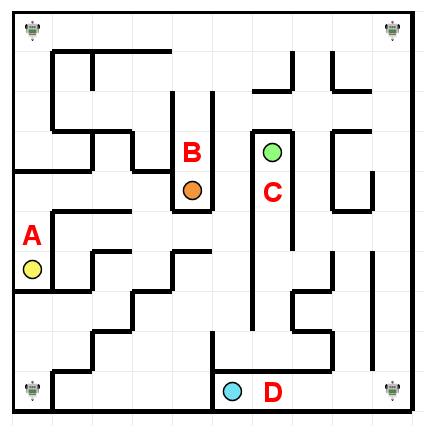
\includegraphics[scale=0.5]{doolhof3}
	\caption{Een van de doolhoven waarop de optimalisatie 6 getest werd.}
\label{fig:TestDead}
\end{figure}

\begin{table}[h]
\begin{center}
    \begin{tabular}{ c | c | c | c | c}
   \multicolumn{2}{c|}{Met optimalisatie 6} & \multicolumn{2}{|c|}{Zonder optimalisatie 6} & \\
     gevonden locatie & afgelegde weg (cm) & gevonden locatie &  afgelegde weg (cm) & verbetering?\\ \hline\hline
    A & 720 & B & 880 & ja \\ \hline
    B & 1520 & D & 2960 & ja \\ \hline
    D & 4320 & C & 4520 & ja\\ \hline
    C & 6120 & A & 5920 & nee\\
    \end{tabular}
    \caption{Testresultaten optimalisatie 6: start linksboven in de doolhof uit figuur \ref{fig:TestDead}}
    \label{tab:resultVerken1}
\end{center}
\end{table}

\begin{table}[h]
\begin{center}
    \begin{tabular}{c | c | c | c | c}
   \multicolumn{2}{c|}{Met optimalisatie 6} & \multicolumn{2}{|c|}{Zonder optimalisatie 6} &\\
     gevonden locatie &  afgelegde weg (cm) & gevonden locatie &  afgelegde weg (cm)& verbetering?\\ \hline\hline
    D & 120 & D & 120 & -\\ \hline
    A & 2920 & A & 2600 & nee\\ \hline
    B & 3720 & B & 3240 & nee\\ \hline
    C & 6240 & C & 6000 & nee\\
    \end{tabular}
    \caption{Testresultaten optimalisatie 6: start rechtsonder in de doolhof uit figuur \ref{fig:TestDead}}
    \label{tab:resultVerken2}
\end{center}
\end{table}

De optimalisatie werd getest door de simulator verschillende keren door vier verschillende doolhoven te laten rijden. De robot startte in elke hoek van elke doolhof zowel met optimalisatie als zonder. De robot dient de tegel met het voorwerp niet echt te bezoeken; het is voldoende de barcode ervoor te lezen om te weten of het om het juiste voorwerp gaat. Dus enkel de afgelegde afstand van het startpunt tot de punten~A,~B, C~en~D is van belang. Tabellen~\ref{tab:resultVerken1} en~\ref{tab:resultVerken2} geven resultaten weer voor de doolhof uit figuur~\ref{fig:TestDead}. Niet alle testresultaten werden weergegeven; het groot aantal tabellen zou weinig meerwaarde bieden.\\

%testresultaten: 25x beter (24,3%); 30x even goed (29,1%); 48x slechter (46,6%)
Een vergelijking van alle testresultaten toont dat het algoritme met deze optimalisatie slechts in 24\% van de gevallen een verbetering is. In 47\% van de gevallen doet de robot er zelfs langer over. Het is immers moeilijk het kortste pad naar de voorwerplocatie te bepalen wanneer de tegels op dat pad nog niet verkend zijn. In dat geval kan het pad enkel op basis van de manhattanafstand geschat worden, zonder de muren in rekening te brengen. Dit zorgt ervoor dat de robot vaak moet terugkeren om een nieuw pad te zoeken. Deze implementatie van de optimalisatie is daarom niet de moeite om toe te voegen aan het algoritme. \\


\subsection{Samenvoegen van doolhoven}
\label{ssec:AlgoMappen}
%TODO beter schrijven
Wanneer een robot zijn voorwerp gevonden heeft, weet hij bij welk team hij hoort. Hij stuurt vanaf dan periodisch zijn map door en kijk regelmatig of zijn teamgenoot een map heeft gestuurd.
Wanneer de robot een map ontvangt gaat hij op zoek naar een paar unieke punten. Dit zijn tegels met een voorwerp en de aangrenzende barcode of tegels met een wip en de aangrenzende barcode. De robot kijkt vervolgens of zijn eigen map dit unieke paar ook bevat. Indien dit niet het geval is, zoekt de robot naar andere unieke paren of wacht hij tot een nieuwe doolhof binnenkomt.
Indien de robot het unieke paar ook in zijn map heeft, kunnen beide mappen worden samengevoegd. E\'en van beide punten van het paar wordt als referentiepunt gekozen. Beide mappen worden verschoven tot dit punt op co\"ordinaat $(0,0)$ ligt. De robot vergelijkt dan de co\"ordinaten van het andere punt uit het unieke paar. Wanneer deze in de twee mappen niet gelijk zijn, wordt de tweede map geroteerd tot de co\"ordinaten van het tweede punt ook samenvallen.

De translaties van beide mappen naar $(0,0)$ en de rotatie van de tweede map leidt tot een algemene transformatiematrix. Deze verandert echter alleen de co\"ordinaten van de tegels, niet de ori\"entatie van de tegels zelf. Wanneer de matrix geroteerd wordt, moeten alle tegels afzonderlijk van ori\"entatie veranderd worden.\\

Wanneer de volledige projectie bepaald is, kan deze elke keer gebruikt worden wanneer een nieuwe doolhof ontvangen worden. Ze hoeft niet opnieuw berekend te worden.

\subsection{Teamgenoot bereiken}
\label{ssec:AlgoAndereRobot}
%TODO geen persoonlijke ventilatie van meningen
De scheidsrechterscommissie besloot dat alle robots informatie doorsturen over hun positie. Naar een teamgenoot stuurt een robot ook zijn volledige map. De teamgenoten rijden dan naar elkaar, zonder expliciet een tegel af te spreken. Wanneer de robots elk een ander pad kiezen, zou het echter kunnen dat ze elkaar kruisen. Deze oplossing lijkt ons daarom niet optimaal, maar we leggen ons neer bij de beslissing.\\

Om naar de juiste plek te gaan gebruikt de robot het kortste pad algoritme.

\subsection{Andere robots}
\subsubsection{Robot-detectie sensor}
\label{ssec:AlgoCollision}
%TODO dit gaat over de hyride sensor gaan. 


% == SOFTWARE == %
\section{Software}
\label{sec:Softw}
De software bestaat uit twee delen: een project dat op de NXT van de robot loopt en een project dat op de computer loopt (sectie~\ref{ssec:Sdesign}). Alles wordt aangestuurd via de \textit{Graphical User Interface (GUI)} (sectie~\ref{ssec:GUI}). Deze laat toe de robot te besturen en de reacties van de robot weer te geven. Robots kunnen met elkaar communiceren via RabbitMQ (sectie~\ref{ssec:RabbMQ}). Via de GUI kunnen ook virtuele robots aangestuurd worden: de simulatoren (sectie~\ref{ssec:Sim}). Tijdens het verkennen wordt een map opgeslagen van de wereld (sectie~\ref{ssec:Mapping}).\\

Voor volgende secties wordt verwezen naar het verslag van het eerste semester. Deze implementaties en ontwerpen werden zonder aanpassingen opnieuw gebruikt:

\begin{itemize}
\item Commando's doorgeven
\item Bluetooth
\item Robot
\end{itemize}

% -- Ontwerp -- %
\subsection{Algemeen software-ontwerp}
\label{ssec:Sdesign}
Een overzicht van het ontwerp wordt weergegeven in figuur~\ref{fig:klasSoft}.\\

% figuren klassendiagramma
\begin{figure}
\centering
		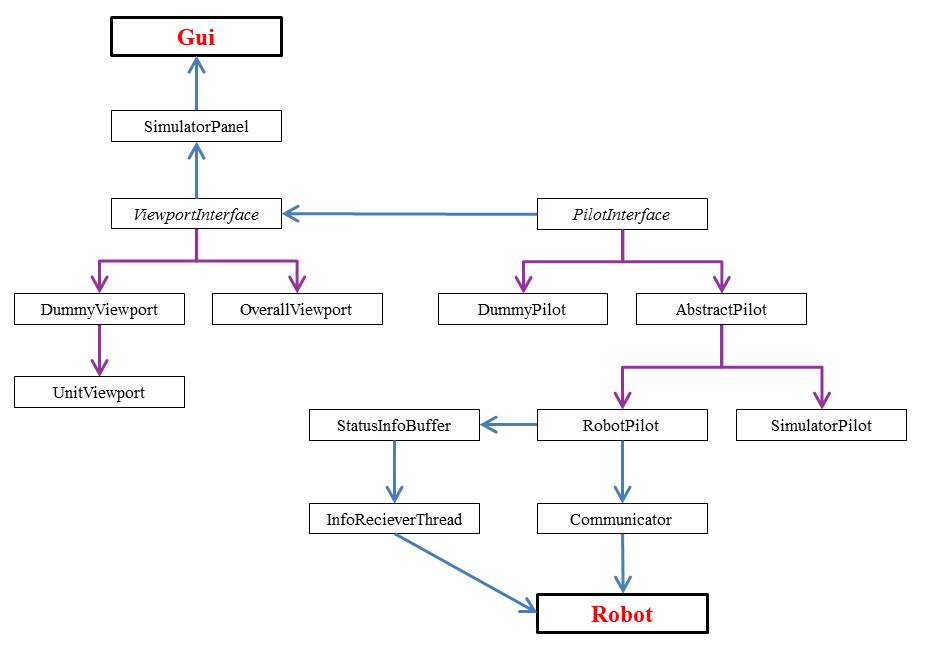
\includegraphics[width=\textwidth]{KlasSoftware}
\caption[Klassendiagram computerproject]{Klassendiagram met de belangrijkste klassen van het computerproject (paarse pijlen wijzen op overerving of implementatie)}
\label{fig:klasSoft}
\end{figure}

De Main-methode bevindt zich in de GUI-klasse. Deze maakt een \textit{SimulatorPanel}-object aan. Dit is een overkoepelend panel waarin meerdere \textit{Viewports} zitten. Een \textit{OverallViewport} geeft het volledige doolhof en alle robots erin weer. Dit kan uiteraard enkel wanneer een gekend virtueel doolhof gebruikt wordt en wanneer van alle robots genoeg informatie beschikbaar is. Een \textit{UnitViewport} geeft de wereld van \'e\'en robot (eventueel gesimuleerd) weer: de sensorwaarden en de muren die hij reeds ontdekt heeft. Een wereld waarvan niets geweten is, kan niet worden weergegeven. Dit is het geval voor robots van andere teams: zij worden niet weergegeven in de GUI, met uitzondering van de teamgenoot. Deze laatste stuurt wel zijn map door, maar niet zijn sensorwaarden en wordt gerepresenteerd door een \textit{DummyViewport}. Het aantal \textit{Viewports} hangt af van het aantal gekende werelden.\\

Een \textit{DummyViewport} is aanvankelijk leeg. Wie de teamgenoot van de robot is, wordt immers pas bekend wanneer beide leden van het team hun voorwerp gevonden hebben. Op dat moment zal de \textit{DummyViewport} iets weergeven.\\

Elke \textit{Viewport} krijgt een eigen \textit{Pilot} toegewezen (behalve \textit{OverallViewport}, die krijgt er meerdere). Een \textit{Pilot} is een implementatie van \textit{PilotInterface}. Er zijn verschillende soorten \textit{Pilots}. De keuze van \textit{Pilot} hangt af van het type robot:

\begin{enumerate}
	\item Een robot waarvan de wereld niet kan worden voorgesteld, krijgt geen \textit{Pilot}.
	\item Een teamgenoot (die we niet zelf simuleren) heeft een \textit{DummyPilot}. Deze bevat enkel `getters', want deze robot kan niet worden aangestuurd.
	\item Een robot die gesimuleerd wordt, heeft een \textit{SimulatorPilot}. Deze berekent zelf zijn sensorwaarden op basis van een virtuele doolhof.
	\item Een fysieke robot krijgt een \textit{RobotPilot} die via de \textit{Communicator} in verbinding staat met de fysieke robot. De \textit{RobotPilot} krijgt zijn sensorwaarden terug van de robot via de \textit{InfoReceiverThread} en de \textit{StatusInfoBuffer}.
\end{enumerate}

 Zowel \textit{SimulatorPilot} als \textit{RobotPilot} erven over van \textit{AbstractPilot}. Dit zijn de `hersenen' van deze robots/simulatoren. De \textit{AbstractPilot} bepaalt hoe de (gesimuleerde) robot moet reageren in de gegeven situatie. De klasse bevat methodes als \textit{travel()} en \textit{rotate()}. Ook bouwt de \textit{AbstractPilot} een map op terwijl de (gesimuleerde) robot zich voortbeweegt door het doolhof.

% -- GUI -- %
\subsection{Grafische User Interface}
\label{ssec:GUI}

% figuur GUI
\begin{figure}[h]
\centering
	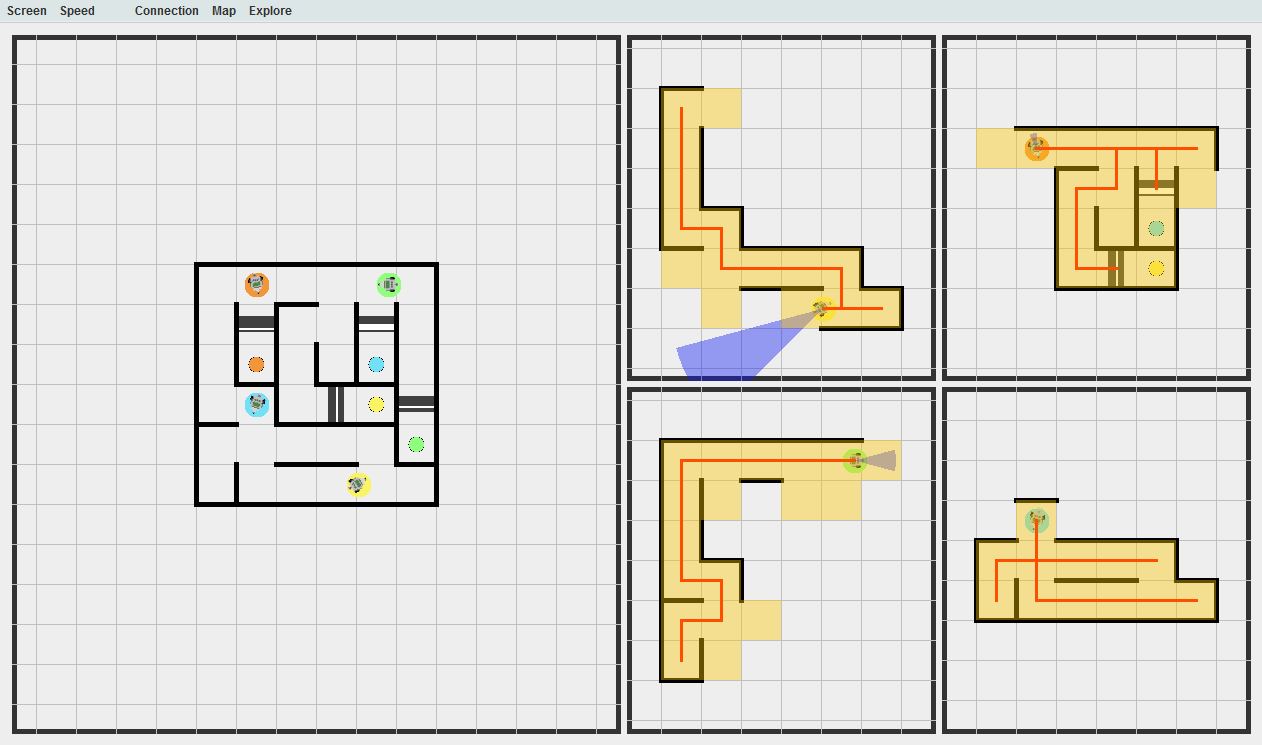
\includegraphics[width=0.8\textwidth]{GUI1}
\caption{de Graphical User Interface met drie gesimuleerde robots}
\label{fig:GUI1}
\end{figure}

% figuur GUI
\begin{figure}[h]
\centering
	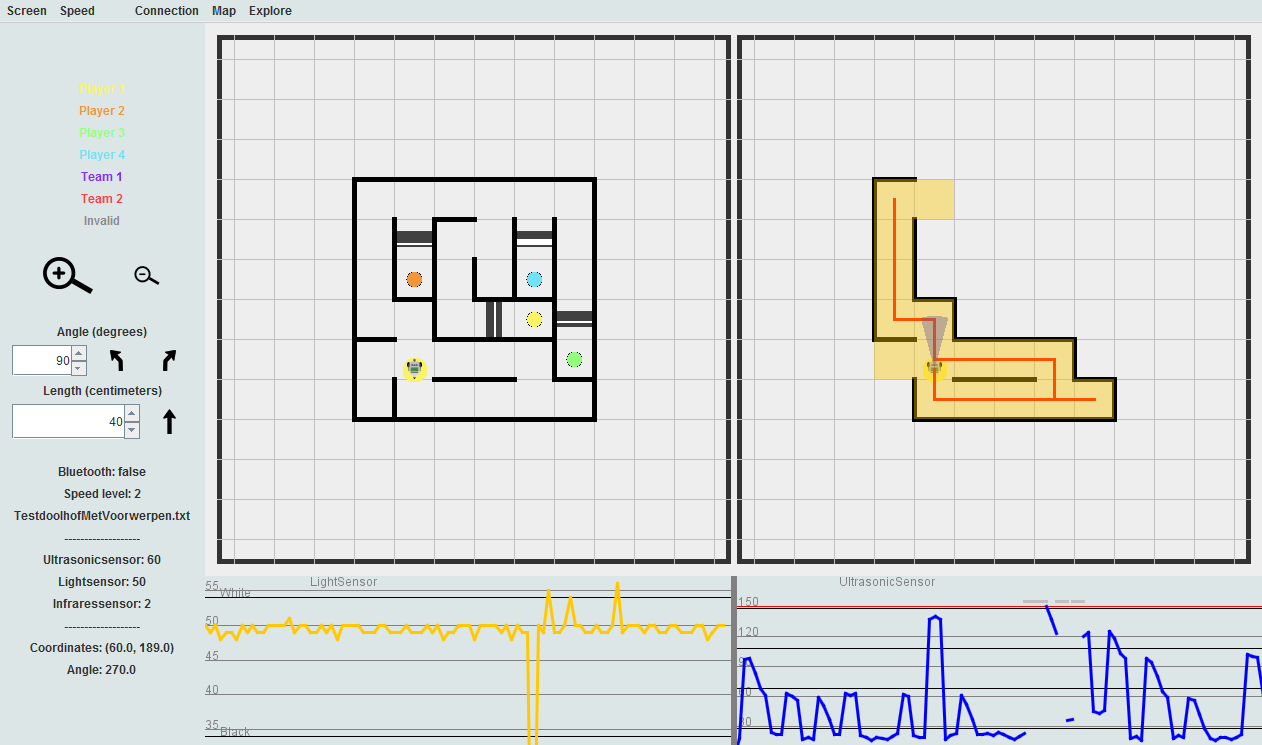
\includegraphics[width=0.8\textwidth]{GUI2}
\caption{de Graphical User Interface met infopanel, inputpanel en sensorgrafieken}
\label{fig:GUI2}
\end{figure}

Figuren~\ref{fig:GUI1} en~\ref{fig:GUI2} tonen de GUI bij verschillende instellingen. De GUI toont links de \textit{OverallVieuwport}: de volledige map met alle robots, voorwerpen en barcodes erin. Elke robot heeft initieel een eigen kleur. Deze kleur komt overeen met het voorwerp dat de robot moet zoeken. Wanneer een robot zijn voorwerp gevonden heeft, verandert zijn kleur in de teamkleur. Op het einde hebben de robots van hetzelfde duo dezelfde kleur.\\

Rechts worden de \textit{UnitViewports} en \textit{DummyViewports} weergegeven. Wanneer de robot een pad aflegt, tekenen de \textit{Viewports} dit als een rode lijn. De huidige positie en de huidige ori\"entatie van de robot worden weergegeven door een figuur die draait met de ori\"entatie. Het bereik van de ultrasone sensor wordt grafisch weergegeven met een blauwe boog. Een \textit{DummyViewport} geeft geen sensorwaarden weer. De map-in-opbouw wordt weergegeven op basis van de map die de \textit{Pilot} opstelt. Alle tegels die in de map zitten worden oranje gekleurd. De robot heeft deze tegels niet altijd bezocht, maar weet wel van hun bestaan af. Dit is handig bij het testen van verkenalgoritmes.\\

Het aantal \textit{UnitViewports} of \textit{DummyViewports} hangt af van de situatie. Dit kan makkelijk worden ingesteld via de menubar. Het is ook mogelijk extra panelen te laten verschijnen die sensorwaarden op een grafiek en in cijfers weergeven. Ook het paneel om de robot handmatig te besturen kan tevoorschijn gehaald wordt via de menubar. Dit is te zien in figuur~\ref{fig:GUI2}.

% -- RabbitMQ -- %
\subsection{Communicatie tussen de robots}
\label{ssec:RabbMQ}
De scheidsrechterscommissie ontwikkelde \textit{Het Team Treasure Trek Protocol (HTTTP)} en een implementatie ervan. De implementatie bevat o.a. een \textit{Client}-klasse die het gebruik van RabbitMQ bijna volledig abstraheert. Ook een \textit{Handler}-interface is voorzien. Deze moet door de teams zelf ge\"implemeteerd worden. Figuur~\ref{fig:klasHTTTP} toont een schema van de implementatie.\\

Het computerproject bevat een \textit{PlayerHandler} en een \textit{SpectatorHandler}, om respectievelijk in de \textit{AbstractPilot} en de \textit{DummyPilot} met informatie om te gaan. Een onderscheid is nodig omdat \textit{DummyPilots} `aangestuurd' worden via hun \textit{Handler}.\\

Bij het aanmaken van een \textit{Pilot} wordt een \textit{MQCenter} aangemaakt met bijhorende \textit{Handler}. Het \textit{MQCenter} abstraheert de \textit{Client}-klasse nog verder.

% klassendiagram HTTTP
\begin{figure}[h]
\centering
	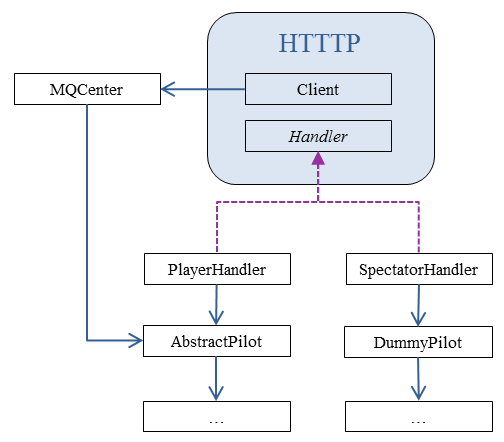
\includegraphics[width=0.5\textwidth]{KlasHTTTP}
\caption{Klassendiagram HTTTP}
\label{fig:klasHTTTP}
\end{figure}


% -- Simulator -- %
\subsection{Simulator}
\label{ssec:Sim}
De \textit{Simulator} bootst de werking van de robot virtueel na. Hij kan dezelfde commando's uitvoeren als de werkelijke robot en simuleert de sensorwaarden die een echte robot zou genereren wanneer deze zich in een soortgelijke situatie bevindt.\\

De \textit{SimulatorPilot} bepaalt de positie van de `robot' ten opzichte van het virtuele doolhof: hoe ver van de muur en op welke ondergrond. De klasse \textit{SimulationSensorData} houdt sensorwaarden bij van tests op de echte robot in verschillende situaties. De \textit{SimulatorPilot} haalt hier zijn referenties uit en probeert op basis van de meetwaarden een realistische sensorwaarde te genereren. De sensorwaarden worden niet nauwkeurig gegenereerd: er wordt ruis toegevoegd. De echte robot geeft immers ook geen exacte waarden.\\

% -- Mapping -- %
\subsection{Mappen van een doolhof} % 3 ok
\label{ssec:Mapping}
Het \textit{Mapping}-pakket bevat objecten die elementen uit de wereld van een robot voorstellen. Figuur~\ref{fig:klasMap} geeft de structuur van het pakket weer. De klasse \textit{MapGraph} brengt al deze elementen samen. Ze biedt functionaliteiten om van de huidige tegel naar een aanliggende tegel te reizen en om de map dynamisch uit te breiden. Zo wordt impliciet een hele graaf bijgehouden. De klasse \textit{MapReader} kan uit een bepaalde textfile een \textit{MapGraph} opstellen.\\

De \textit{SimulatorPilot} heeft een \textit{MapGraph} die de virtuele doolhof voorstelt. Tijdens het verkennen wordt een nieuwe \textit{MapGraph} opgesteld door de \textit{AbstractPilot}. Deze bevat enkel informatie die de robot zelf verzamelde.

% klassendiagram mapping
\begin{figure}[h]
\centering
	\includegraphics[width=0.8\textwidth]{klasMapping}
\caption{Klassendiagram mapping}
\label{fig:klasMap}
\end{figure}


% == BESLUIT == %
\section{Besluit}
\label{sec:Besluit}
De bouw van de robot wordt uitgebreid met een infraroodsensor. De schep vooraan wordt aangepast en van klittenband voorzien. Zowel de schep als de lichtsensor zijn gemonteerd op een hefboomsysteem dat omhoog klapt wanneer het de wip raakt. Zo geraakt de robot makkelijk de wip op.\\

Er kunnen verschillende robots worden gesimuleerd of gemodelleerd. Al deze robots hebben een eigen idee van de wereld. Deze verschillende werelden worden weergegeven via \textit{Viewports}. Een \textit{OverallViewport} toont de werkelijke wereld en alle robots erin.\\

De robot communiceert met andere robots via RabbitMQ. Zo kan de robot afspraken maken met anderen en kan hij te weten komen wie zijn teamgenoot is.


\newpage
\makeappendix

%%% == DEMO 1 == %
%\section{Demo 1} % 3
%\label{Asec:demo1}
%De robot wordt voor de eerste demo voorzien van een schep die bestaat uit een halve wc-rol. De infraroodsensor is ge\"installeerd, maar wordt nog niet gebruikt. Wanneer de robot zijn voorwerp vindt, stuurt hij een bericht via RabbitMQ. De GUI is opgesplitst in verschillende \textit{Viewports} die elk een of meerdere \textit{Pilots} weergeeft.
%
%% == resulaten == %
%\subsection{Resultaten} % 3 ?
%\label{Assec:result1}
%Het algoritme waarmee de robot zijn voorwerp opraapte, maakte gebruik van de travel() methode. De \textit{ExploreMaze}-thread wist echter niet dat de robot van plek was veranderd. In de waan dat de robot op een andere plek stond dan in werkelijkheid, gaf de thread verkeerde instructies waardoor de robot tegen een muur reed. \\
%Het schepsysteem van de robot functioneerde niet. Tijdens de demo faalde de robot toen hij het object moest oprapen. 
%
%% == conclusies == %
%\subsection{Conclusies} % 3 ?
%\label{Assec:conc1}
%Het bovengenoemd probleem is voor de volgende demo opgelost. Wanneer de \textit{ExploreMaze}-thread onderbroken wordt, zorgt de onderbrekende methode steeds dat de robot op dezelfde plek staat als waar de \textit{ExploreMaze}-thread denkt dat de robot staat.\\
%De schep is ook aangepast. De schep is weggehaald en er is een klittenband aangebracht. De robot is nog steeds in staat om het voorwerp met een scharnierend systeem op te heffen, zodat de robot vlot over de wip heen kan.
%
%
%% == aanpassingen == %
%\subsection{Oplijsting aanpassingen verslag} % 3 ?
%\label{Assec:aanp1}
%Volgende secties werden aangepast ten opzichte van de eerste demonstratie van het tweede semester:
%
%% overzicht aangepaste secties
%\begin{itemize}
%\item \textit{\ref{ssec:Abstract} Samenvatting:} aangepast.
%\item \textit{\ref{ssec:FysB} Fysieke bouw:} de schep vooraan.
%\item \textit{\ref{ssec:AlgoZoek} Zoeken van het voorwerp:} testen van de prioriteit.
%\item \textit{\ref{ssec:AlgoAndereRobot} Weg vinden naar teamgenoot:} nieuwe sectie.
%%\item \textit{\ref{ssec:AlgoMappen} Twee mappen samenvoegen:} nieuwe sectie.
%\item \textit{\ref{ssec:GUI} Grafische User Interface:} nieuwe figuren en aangepaste tekst.
%\item \textit{\ref{ssec:RabbMQ} Communicatie via RabbitMQ:} implementatie \textit{HTTTP}.
%\item \textit{\ref{ssec:Mapping} Mappen van een doolhof:} wip en voorwerpen toegevoegd.
%\end{itemize}

%% == DEMO 2 == %
\section{Demo 2}
\label{Asec:demo2}
Voor de tweede demonstratie wordt er met \'e\'en fysieke en drie gesimuleerde robots gewerkt. Het is ook de bedoeling om  met vier virtuele robots te werken. Het doolhof bevat mogelijk een wip. De robots zijn in staat hun eigen voorwerp te vinden en op te rapen. Nadat de robot zijn eigen voorwerp heeft opgeraapt communiceert hij dit en vraagt wie zijn teamgenoot is. Wanneer een robot weet wie zijn teamgenoot is, kan hij hiermee een punt afspreken om samen te komen.\\

% == resulaten == %
\subsection{Resultaten}
\label{Assec:result2}
Het verkennen van de doolhof gebeurde volledig zoals het hoorde. De robot was enkele dagen voor de demonstratie terug gekalibreerd en reed heel nauwkeurig. Het nemen van de wip lukte niet doordat de robot bleef haken met zijn lichtsensor aan de opstap van de wip.\\
De robot slaagde er niet in zijn voorwerp te vinden. Ook het samenvoegen van twee mappen was niet mogelijk.\\
De simulator van de robot was wel in orde. Het was mogelijk om 4 robots te simuleren. Het enige minpuntje zat hem in de visualisatie van het pad. Er zaten discontinu"iteiten in waardoor er shocken zaten in de visualisatie van het pad. \\

% == conclusies == %
\subsection{Conclusies}
\label{Assec:conc2}
De demo ging zeker niet zoals het zou moeten. We hebben niet kunnen demonstreren hoe de robot het voorwerp zou oprapen. Ook het samenvoegen van de twee mappen was niet mogelijk. Toen de robot het doolhof verkende ging het zeer goed tot op het moment dat de robot een wip op moest gaan. De robot bleef haken waardoor de robot uiteindelijk crashte. Voor de volgende demo gaan we er voor zorgen dat de discontinu"iteit in de visualisatie van het pad verdwenen is en dat de robot geen problemen meer ondervindt met het opgaan van de wip.


% == aanpassingen == %
\subsection{Oplijsting aanpassingen verslag}
\label{Assec:aanp2}
Volgende secties werden aangepast ten opzichte van de eerste demonstratie van het tweede semester:

%TODO
% overzicht aangepaste secties
\begin{itemize}
\item \textit{\ref{ssec:FysB} Ontwerp:} nieuwe bouw.
\item \textit{\ref{ssec:Kalib} Kalibratie:} nieuwe sectie.
\item \textit{\ref{ssec:AlgoAllign} De robot aligneren:} nieuw algoritme.
\item \textit{\ref{ssec:AlgoBar} Kalibratie:} nieuw algoritme.
\item \textit{\ref{ssec:AlgoWip} Omgaan met de wip:} nieuwe sectie.
%\item \textit{\ref{ssec:AlgoAndereRobot} Weg vinden naar teamgenoot:} aangepast.
\item \textit{\ref{ssec:AlgoMappen} Twee doolhoven samenvoegen:} nieuwe sectie.
\item \textit{\ref{ssec:AlgoCollision} Botsingen met andere robots vermijden:} nieuwe sectie.
\item \textit{\ref{ssec:GUI} Grafische User Interface:} nieuwe figuren en aangepaste tekst.
\end{itemize}


\begin{thebibliography}{9}

\bibitem{TeamTreasure} 
\textit{Team Treasure Trek}: Een onderdeel van Mario Party 4. \mbox{[www.nintendo-europe.com/]}

\bibitem{RabbitMQ}
\textit{RabbitMQ}: Een communicatiesysteem dat het Advanced Message Queing Protocol (AMQP) implementeert. Door een kanaal op te zetten met een RabbitMQ-server is het mogelijk een bericht te plaatsen dat anderen kunnen lezen. De server heeft enkele `exchanges' die de berichten verdelen over `queues'. Die `queues' worden aangemaakt door de `clients' en luisteren elk naar een bepaald onderwerp. De `exchange' pushed dus berichten met een bepaald onderwerp naar de juiste `queues'.
\mbox{[http://en.wikipedia.org/wiki/RabbitMQ]}

\bibitem{mindstorms}
\textit{Lego Mindstorms}:  Een uitbreiding op de LEGO bouwstenen waarmee kleine, aanpasbare en programmeerbare robots gebouwd kunnen worden. Een centrale besturingsmodule (`the brick') kan geprogrammeerd worden met verschillende programmeertalen. In eerdere versies werd een RCX gebruikt voor de brick, nu wordt met NXT gewerkt. De brick kan enkele motoren aandrijven. Bovendien kunnen er verschillende sensoren, o.a. een ultrasone sensor en een lichtsensor, aangesloten worden.  \mbox{[www.lego.com]} \mbox{[http://en.wikipedia.org/wiki/Lego\textendash Mindstorms]}

\bibitem{leJOS}
\textit{leJOS}: Een kleine Java Virtuele Machine die toelaat de NXT-brick te programmeren. leJOS voorziet verschillende klassen die o.a. de motoren aansturen en een bluetoothverbinding opzetten.  \mbox{[http://lejos.sourceforge.net/]}



\end{thebibliography}


\end{document}
